
%\VignetteIndexEntry{SynthEx Vignette}
%\VignetteKeyword{Whole exome sequencing}
%\VignetteKeyword{Targeted sequencing}
%\VignettePackage{SynthEx}

\documentclass{article}
\RequirePackage[]{/Library/Frameworks/R.framework/Versions/4.0/Resources/library/BiocStyle/resources/tex/Bioconductor}
\AtBeginDocument{\bibliographystyle{/Library/Frameworks/R.framework/Versions/4.0/Resources/library/BiocStyle/resources/tex/unsrturl}}
\usepackage[noae, nogin]{Sweave}
\usepackage{graphicx}
\usepackage{amsmath}
\usepackage{times}
\usepackage{listings}

\lstset{basicstyle=\ttfamily,
  language=bash,
  showstringspaces=false,
  commentstyle=\color{red},
  keywordstyle=\color{blue},
  morekeywords={cut,paste,sort,samtools}
}

\newcommand{\pkg}[1]{\texttt{\textsl{#1}}}
\newcommand{\code}[1]{\texttt{#1}}



\author{Mengjie Chen}
\title{SynthEx}


\usepackage{Sweave}
\begin{document}
\Sconcordance{concordance:SynthEx-knitr.tex:SynthEx-knitr.Rnw:%
1 6 1 1 2 1 0 1 2 16 1 1 7 6 1 1 0 24 1 1 4 6 1 1 4 8 1 1 2 1 0 6 1 1 2 %
1 0 2 1 3 0 1 2 1 1 1 2 1 0 2 1 3 0 1 2 1 4 4 1 1 2 4 0 1 2 3 1 1 2 1 0 %
3 1 1 4 7 0 1 3 3 1 1 2 4 0 1 2 2 1 1 2 1 0 2 1 24 0 1 2 1 1 1 8 4 1 1 %
2 1 0 1 1 3 0 1 2 2 1 1 2 1 0 2 1 3 0 1 2 2 1 1 7 9 0 1 2 1 1 1 2 1 0 1 %
4 6 0 1 2 4 1 1 2 1 0 1 1 1 7 9 0 1 2 42 1 1 2 1 0 4 1 11 0 1 1 12 0 1 %
2 3 1 1 7 9 0 1 2 10 1 1 2 1 0 2 1 1 6 8 0 1 2 14 1 1 2 4 0 1 2 1 11 13 %
0 1 2 16 1 1 2 1 0 1 7 9 0 1 2 15 1 1 9 8 0 1 3 4 0 1 2 12 1 1 4 6 0 1 %
2 3 1 1 4 6 0 1 2 6 1 1 2 1 0 1 2 1 0 3 1 1 6 5 0 1 3 2 0 1 1 1 3 5 0 1 %
2 8 1 1 2 1 0 1 6 5 0 1 5 7 0 1 2 13 1 1 2 1 0 2 1 1 5 4 0 1 6 5 0 1 6 %
8 0 1 2 10 1 1 2 1 0 2 1 12 0 1 2 1 7 6 0 1 7 6 0 1 5 7 0 1 2 2 1 1 2 1 %
0 1 6 8 0 1 2 10 1 1 4 6 0 1 2 4 1 1 3 2 0 1 5 7 0 1 2 2 1 1 4 3 0 1 1 %
3 0 1 2 5 1}


\maketitle

  \vspace{1em}

  \textbf{SynthEx version:} 1.6

  \vspace{1em}

  \begin{center}
    \begin{tabular}{ | l | }
      \hline
     Please cite:  \\
     Grace O. Silva, Marni Segal, Xiaping He, Lisle E. Mose, Joel S. Parker, \\
     Wei Sun, Charles M. Perou and Mengjie Chen \\
     SynthEx: Capture-specific, ``synthetic''-normal based whole exome/genome sequencing tool \\
     for copy number alteration detection and tumor heterogeneity profiling. \\
      Genome Biol. 2017;18(1):66. Published 2017 Apr 8. doi:10.1186/s13059-017-1193-3 \\
      \hline
    \end{tabular}
  \end{center}



\newpage

\tableofcontents

\newpage


\section{Introduction of package \pkg{SynthEx}}
\pkg{SynthEx} is a comprehensive suite of tools for CNA detection and tumor heterogeneity profiling. It is tailored to cater for the multiple characteristics of different next generation sequencing technologies. \pkg{SynthEx} is the first method aware of the sample-specific bias in targeted regions due to fold enrichment differences in tumor and normal samples. Fundamentally different from current methods, it applies different analytical strategies for single subject and large-scale cancer genomics studies. For large-scale cancer genomics studies, it corrects the technical bias due to capture efficiency by using a ``synthetic''-normal strategy. The ``synthetic''-normal samples were generated by stratifying existing normal samples (including samples outside the current study) based on capture protocols. Therefore, instead of requiring a matched pair normal sample from each tumor subject, a ``synthetic" normal is used that mimics the targeted sequencing profile with the same capture efficiency level as the tumor sample. This strategy can potentially reduce both the experiment and analysis burden within a sequencing facility. In addition, since ``synthetic'' normals can be used for any tumor samples processed by the same protocol, they can be used to analyze mouse xenograft samples or cell line samples, paired normals of which are traditionally difficult and even impossible to obtain.

\pkg{SynthEx} can be used to analyze whole exome sequencing, targeted sequencing and whole genome sequencing data.

\section{Installation}
\pkg{SynthEx} relies on the following R packages: \pkg{mclust}, \pkg{flsa}, \pkg{foreach}, \pkg{DNAcopy}, \pkg{ggplot2}, \pkg{gridExtra}, \pkg{inline}, and \pkg{Rcpp}.

\begin{Schunk}
\begin{Sinput}
 install.packages("mclust")
 install.packages("flsa")
 install.packages("foreach")
 install.packages("ggplot2")
 install.packages("gridExtra")
 install.packages("inline")
 install.packages("Rcpp")
 if (!requireNamespace("BiocManager", quietly = TRUE))
     install.packages("BiocManager")
 BiocManager::install()
 BiocManager::install("DNAcopy")
\end{Sinput}
\end{Schunk}

\pkg{SynthEx} can be installed directly from github.
\begin{Schunk}
\begin{Sinput}
 install.packages ("devtools")
 library(devtools)
 install_github("ChenMengjie/SynthEx")
\end{Sinput}
\end{Schunk}


\section{Pre-processing and preparation}

\pkg{SynthEx} takes counts data in non-overlapping genomic bins from tumor and normal samples as input. It has the option to input variant calling results from tumor sample. Thus \pkg{SynthEx} relies on other tools to generate appropriate input files. We recommend \pkg{BEDtools} for getting the bin-level count data and \pkg{freebayes} for variant calling. In addition, \pkg{SynthEx} calls the \code{intersectBed} function from \pkg{BEDtools} directly, so \pkg{BEDtools} should be installed.
Linux or Mac users can obtain the directory of \code{intersectBed} by running:
\begin{Schunk}
\begin{Sinput}
 intersectBed.dir <- system("which intersectBed", intern=TRUE)
\end{Sinput}
\end{Schunk}
If it doesn't work on your system, you need to specifiy \code{intersectBed.dir} manually.


When evaluating sample bias at targeted regions, it requires annotations for targets. The annotations of targeted regions for SureSelect are pre-installed \pkg{SynthEx} and will be used as the default if annotations are not specified by users. All bins will be classified into two categories: target bins, if overlapped with any selectively amplified targets, and off-target bins, otherwise. Such classification is pre-calculated for hg19 genome with 10kb, 25kb, 50kb and 100kb. If using bin size not listed here or other annotation, users need to provide such a file or generate such as file by running \code{createTargetBins()}.
\begin{Schunk}
\begin{Sinput}
 library(SynthEx)
 data("TargetAnnotations")
 head(TargetAnnotations$bin100000)
 head(TargetAnnotations$Target)
 targetAnnotateBins <- createTargetBins(
     TargetAnnotations$Target,
     bin.size = 1000000
 )
 
\end{Sinput}
\end{Schunk}

Each row represents a target. First three columns represent chromosome, start and end of a target and last three columns represent chromosome, start and end of its corresponding bin.
Users can choose to remove centromere regions when segmenting the genome. Similarly such information is pre-calculated for hg19 genome with 10kb, 25kb, 50kb and 100kb. If using bin size not listed here or other annotation, users need to provide such a file or generate such as file by running \code{createCentromereBins()}.

\begin{Schunk}
\begin{Sinput}
 centromereBins <- createCentromereBins(bin.size = 10000)
\end{Sinput}
\end{Schunk}

\subsection{Example Data}
\code{TCGAbreast} contains the count data from tumor and its paired normal of TCGA breast cancer samples with bin size of 100kb.
\begin{Schunk}
\begin{Sinput}
 library(SynthEx)
 data(TCGAbreast)
 Lookup(TCGAbreast, show = 6)
\end{Sinput}
\begin{Soutput}
[1] "No.1 element is tumor:"
   chr  start    end TCGA-A1-A0SM TCGA-A2-A04P TCGA-A2-A04Q
1 chr1      0 100000          369         3502          189
2 chr1 100000 200000          153          274           24
3 chr1 200000 300000           79           58           63
4 chr1 300000 400000            4            4            6
5 chr1 400000 500000            4            0            0
6 chr1 500000 600000          389          138          111
[1] "No.2 element is normal:"
   chr  start    end TCGA-A1-A0SM TCGA-A2-A04P TCGA-A2-A04Q
1 chr1      0 100000          568         3135          322
2 chr1 100000 200000           22          481           40
3 chr1 200000 300000           14          224           92
4 chr1 300000 400000            0            6            6
5 chr1 400000 500000            2            0            2
6 chr1 500000 600000          101          411          152
[1] "No.3 element is samples:"
[1] "TCGA-A1-A0SM" "TCGA-A2-A04P" "TCGA-A2-A04Q" "TCGA-A2-A04T" "TCGA-A2-A04X"
[6] "TCGA-A2-A0CM"
\end{Soutput}
\end{Schunk}
\code{Lookup()} is a helper function to take a peek at all elements from a list.


\section{Quick Start}

First specify the directory to save intermediate and final results. If not specified, the default is the current working directory.

\begin{Schunk}
\begin{Sinput}
 working.dir <- ".../working/directory/"
 result.dir <- ".../directory/to/save/results"
\end{Sinput}
\end{Schunk}

\subsection{Single subject analysis}
The input of single subject analysis is names of two BED files or two matrices in BED format that store the count data for tumor sample and its matched normal. Examples can be found in folder \code{ExampleFiles}.
\begin{Schunk}
\begin{Sinput}
 tumor.file <- "./ExampleFiles/TCGA-A7-A26G.tumor.bed"
 normal.file <- "./ExampleFiles/TCGA-A7-A26G.normal.bed"
 sample.name <- "TCGA-A7-A26G"
\end{Sinput}
\end{Schunk}
\code{SynthExPipeline()} is the major funtion that implements the entire \pkg{SynthEx} pipeline. Details about the steps in the pipeline can be found in following sections.

To run segmentation without genotype information, set \code{genotype.file=NULL}.
\begin{Schunk}
\begin{Sinput}
 Segfrompipe <- SynthExPipeline(tumor.file, normal.file,
          bin.size = 100000, intersectBed.dir,
          genotype.file=NULL,
          result.dir, working.dir,
          prefix = sample.name,
          verbose = TRUE)
\end{Sinput}
\end{Schunk}

With genotype information, \pkg{SynthEx} can further estimate purity.
\begin{Schunk}
\begin{Sinput}
 genotype.file <- "./ExampleFiles/TCGA-A7-A26G.freebayes.vcf"
 Segfrompipe <- SynthExPipeline(tumor.file, normal.file,
     bin.size = 100000, intersectBed.dir,
     genotype.file, result.dir, working.dir,
     prefix = sample.name, verbose = TRUE)
\end{Sinput}
\end{Schunk}
The CNA calling results are saved in BED files as \code{'prefix'$\_$Copynumber.bed} and \code{'prefix'$\_$Event.bed}.

\subsection{Multiple subjects analysis}

\pkg{SynthEx} implements a synthetic normal approach, which untilizes normal samples sequenced by the same protocol to reduce unwanted variation due to the sequencing process from tumor samples. To use this approach, \pkg{SynthEx} requires the input of the count data of a tumor sample and multiple normal samples.
\begin{Schunk}
\begin{Sinput}
 tumor.file <- "./ExampleFiles/TCGA-A7-A26G.tumor.bed"
 multiple.normal.file <- "./ExampleFiles/multiple.normal.samples.bed"
 Segfrompipe <- SynthExPipeline(tumor.file,
                                multiple.normal.file,
                                bin.size = 100000,
                                intersectBed.dir,
                                genotype.file,
                                result.dir, working.dir,
                                verbose = TRUE)
\end{Sinput}
\end{Schunk}


\subsection{Generate Data from BAM files}
The count data can be generated from BAM files using standard tools such as \pkg{BEDtools}. The following is an example command to generate count data of a given bin size for one sample using \pkg{BEDtools-2.15.0}:

\begin{lstlisting}
samtools view -h -b -q 10 $bamdir | \
        $bedToolsdir/bin/coverageBed -counts \
        -split -abam stdin -b $chrbinFile > $outdir/sample.$binsize.bed;

sort -k1,1 -k2,2n $outdir/sample.$binsize.bed -o $outdir/sample.$binsize.bed
\end{lstlisting}

The count data for a collection of normal samples can be generated by merging the above count files together using a combination of unix commands, for example:
\begin{lstlisting}
awk -F'\t' 'NR==FNR{a[FNR]=$0;next}{a[FNR]=a[FNR]FS$4} \
  END{for(i=1;i<=FNR;i++)print(a[i])}' \
  $(cat $normallist | xargs -i echo "$sampledir/{}/sample.$binsize.bed") \
  > $outputdir/normal_sample.$binsize.combine.chr.bed


\end{lstlisting}

or

\begin{lstlisting}
awk -F'\t' '{a[FNR]=(a[FNR]?a[FNR]FS:"")$4}END{for(i=1;i<=FNR;i++)print(a[i])}' \
  $(cat $normallist | xargs -i echo "$sampledir/{}/sample.$binsize.bed") \
  > $outputdir/normal_sample.$binsize.combine.bed

cut -f1-3 $sampledir/$firstsample/sample.$binsize.bed \
  | paste - $outputdir/normal_sample.$binsize.combine.bed \
  > $outputdir/normal_sample.$binsize.combine.chr.bed
\end{lstlisting}

where \code{normallist} is the list of normal samples.

\section{Whole exome or targeted sequencing analysis}

\subsection{Single subject analysis}

\subsubsection{Input}
The input of single subject analysis is the names of two BED files or two matrices in BED format.
\begin{Schunk}
\begin{Sinput}
 data(TCGAbreast)
 tumor <- TCGAbreast$tumor[, c(1:3, 11)]
 normal <- TCGAbreast$normal[, c(1:3, 11)]
 sample.name <- TCGAbreast$samples[11]
 head(tumor)
\end{Sinput}
\begin{Soutput}
   chr  start    end TCGA-A2-A0D1
1 chr1      0 100000         2534
2 chr1 100000 200000           57
3 chr1 200000 300000           48
4 chr1 300000 400000            6
5 chr1 400000 500000            0
6 chr1 500000 600000           40
\end{Soutput}
\begin{Sinput}
 head(normal)
\end{Sinput}
\begin{Soutput}
   chr  start    end TCGA-A2-A0D1
1 chr1      0 100000         1555
2 chr1 100000 200000          188
3 chr1 200000 300000          200
4 chr1 300000 400000           10
5 chr1 400000 500000            2
6 chr1 500000 600000           62
\end{Soutput}
\end{Schunk}

\subsubsection{Correct bias in targeted regions}
Given a pair of tumor and matched normal, \pkg{SynthEx} will analyze the sample-specific bias in targeted regions due to fold enrichment differences in tumor and normal samples. \pkg{SynthEx} classifies adjacent bins into either: two adjacent off-target bins, two adjacent targeted bins or an off-target bin next to a targeted bin (Figure 1a). For every pair of adjacent bins we calculate a ratio distance (RD), the difference of read ratio between target and off-target bins, and obtained three main distribution categories. When the ratios in the target and off-target bins follow the same distribution, the density of the RD from a target bin and adjacent off-target bin centralizes at 0 and has the same shape as that from two adjacent target bins or two adjacent off-target bins.

\begin{Schunk}
\begin{Sinput}
 ratioCorrectedBias <- SynthExcorrectBias(tumor, normal,
                bin.size = 100000, rm.centromere = TRUE,
                targetAnnotateBins = NULL, saveplot = FALSE,
                centromereBins = NULL, chrX = FALSE,
                plot = TRUE, result.dir,
                prefix = sample.name, reads.threshold = 25)
\end{Sinput}
\end{Schunk}

\begin{figure}
\begin{center}
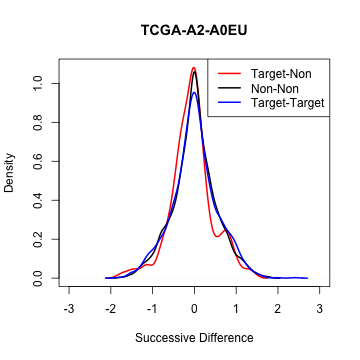
\includegraphics[width=.5\textwidth]{figure/fig1-1}
\end{center}
\caption{An example density plot of RD for three different categories.}
\label{fig:1}
\end{figure}

After running \code{SynthExcorrectBias()}, a density plot for the distances from three categories of adjacent bins will be generated. \pkg{SynthEx} directly uses the mean of RD as an estimator of the bias and de-bias by subtracting it from the observed ratios in target bins. Naturally, the mean and variance of RD can be used as diagnostic metrics to identify ill-behaved samples. As we shown in the paper, the bias in targted regions is due to the differences in fold enrichment of tumor and paried normal sample. The following is an example demonstrating the existence of such bias. Correcting the bias in targeted regions is neccessary when we leverage the information in both target and non-target regions. The following shows an example with such bias in target regions.

\begin{Schunk}
\begin{Sinput}
 tumor <- TCGAbreast$tumor[, c(1:3, 22)]
 normal <- TCGAbreast$normal[, c(1:3, 22)]
 sample.name <- colnames(TCGAbreast$tumor)[22]
 ratioCorrectedBias <- SynthExcorrectBias(tumor, normal,
                bin.size = 100000, rm.centromere = TRUE,
                targetAnnotateBins = NULL, saveplot = FALSE,
                centromereBins = NULL, chrX = FALSE,
                plot = TRUE, result.dir,
                prefix = sample.name, reads.threshold = 25)
\end{Sinput}
\end{Schunk}

\begin{figure}
\begin{center}
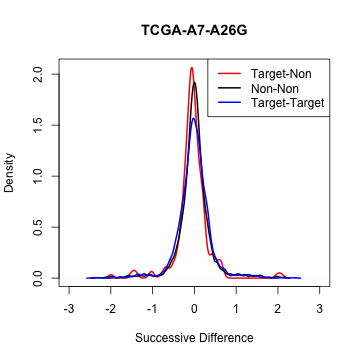
\includegraphics[width=.5\textwidth]{figure/fig2-1}
\end{center}
\caption{Another example density plot of RD for three different categories.}
\label{fig:2}
\end{figure}

\subsubsection{Normalization}

After correcting bias in targeted regions, \pkg{SynthEx} will identify the baseline for copy neutral events.
Most existing methods use median normalization to identify copy neutral regions. The underlying assumption for this strategy is that most regions in the genome are diploid, which does not hold for samples with aneuploidy, such as whole genome doubling. We identify the diploid genome within the tumor sample by gauging information from allele frequencies of heterozygous sites. Specifically, we calculate the median minor allele frequency (MAF) for each bin and select all bins with median MAF greater than 0.45 as candidate copy neutral events (theoretically diploid regions have mean MAF of 0.5). The possible copy number for these bins are 2, 4 and other multiples of 2. To identify diploid bins, we fit a gaussian mixture model for read ratio (RR) and use Bayesian Information Criteria (BIC) to determine the number of copy number state. Finally we assign the mixture component with the smallest mean RR as diploid. The RR in all bins will be adjusted so that diploid regions have expected RR equal to 1.

We use \code{freebayes} to call the variants from tumor samples. A python script within \pkg{SynthEx} can scan all the variants in a VCF file output by \code{freebayes} and select SNPs with MAF greater than 0.05 and supporting reads greater than a threshold (specified by option \code{cutoff}, default is 20). An example VCF file can be found in folder \code{ExampleFiles}. Due to the space limit, we only show the first 200,000 rows of the \code{freebayes} output.
\begin{Schunk}
\begin{Sinput}
 genotype.file <- "./ExampleFiles/TCGA-A7-A26G.freebayes.vcf"
\end{Sinput}
\end{Schunk}

\begin{Schunk}
\begin{Sinput}
 ratioNormalized <- normalization(ratioCorrectedBias,
                                  intersectBed.dir,
                                  genotype.file,
                                  vcf = TRUE,
                                  working.dir,
                                  result.dir,
                                  cutoff = 20,
                                  plot = TRUE,
                                  saveplot = FALSE,
                                  prefix = sample.name)
\end{Sinput}
\end{Schunk}

VCF files generated by other tools can also been processed by the provided python script if they report genotype, read depth and depth of one allele for each variant through "GT", "DP" and "RO", respectively. As an alternative, the author can input non-vcf file with preprocessed SNPs when setting \code{vcf = FALSE}. This require the input in BED format. Example BED files can be found in folder \code{ExampleFiles} (as \code{example.genotype.bed}).

\begin{figure}
\begin{center}
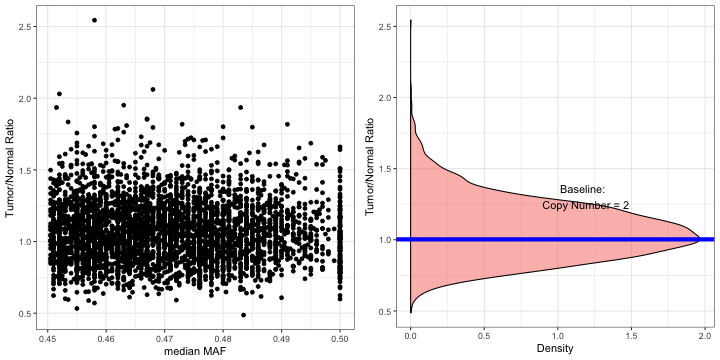
\includegraphics[width=\textwidth]{figure/normalization-1}
\end{center}
\caption{Estimating baseline for copy neutral events using genotype information.}
\label{normalization}
\end{figure}


\code{normalization()} will create a density plot for bins with median MAF greater than 0.45 and indicate the estimated baseline of diploid genome. Normalization step is optional. If genotype data is not provided, median normalization will be used. We strongly recommend to include normalization step if the purpose is to estimate ploidy or call integer copy number.

\subsubsection{Segmentation}

The default segmentation method in \code{SynthEx} is Circular Binary Segmentation (CBS) with default parameters. In this method, CNA signals are modeled as normal random variables with shifts in mean. However, this assumption may not hold due to sequencing biases. A nonparametric model without assuming normality may be more precise. Thus we implement an alternative trending filtering procedure. SynthEx also implements a third segmentation method, SomatiCA, which adds denoising and model selection procedure to CBS. We recommend users to test all three methods on their datasets. Based on our own experience, trending filtering works best on WGS data and SomatiCA works best on WXS data.
\begin{Schunk}
\begin{Sinput}
 Seg <- createSegments(ratioNormalized, "CBS")
 #createSegments(ratioNormalized, "TrendFiltering")
 #createSegments(ratioNormalized, "SomaticaEx", smoothk = 10)
 Segments <- singleCNreport(Seg, report = FALSE,
    result.dir, saveplot = TRUE,
    prefix = sample.name, plotNormalized = TRUE,
    WGD = 1.35, pos.prop.threhold = 0.6,
    pos.log2ratio.threhold = 0.75)
\end{Sinput}
\end{Schunk}
\code{singleCNreport()} can generate a visulization of the segmentation result. When \code{report = TRUE}, \code{singleCNreport()} will write the result into a file named \code{paste0(prefix, "-Segment-", segmentMethod, "-", bin.size, ".txt")}. Users can apply option \code{saveplot = TRUE} to save the plot into a jpg file instead of shown on the screen. In addition, \code{SynthEx} will report whole genome doubling event. The criteria for a whole genome doubling call is either the ploidy greater than \code{WGD} $\times$ 2 or the proportion of positive segments greater than \code{pos.prop.threhold}) and the mean log2 ratio greater than \code{pos.log2ratio.threhold}.


\begin{figure}
\begin{center}
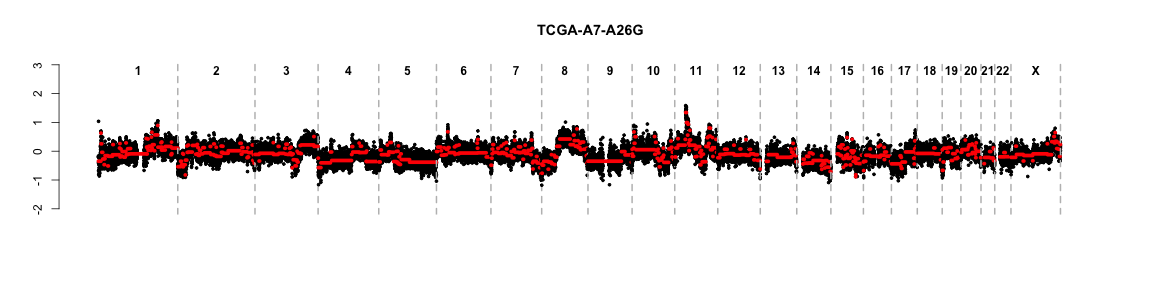
\includegraphics[width=\textwidth]{figure/seg1-1}
\end{center}
\caption{An example for segmentation}
\label{segmentation}
\end{figure}


\subsubsection{Purity estimation}

Accurate estimation of purity is a prerequisite for the quantization of integer level copy number and the clonality analysis. We implement an approach with the following core idea: the proportion of intermixed normal cells can be estimated from the shift of copy ratios of clonal CNAs from their expectations in the pure homogeneous tumor sample. In this approach, we first used spectral clustering (option \code{tau} specifies the free parameter in Gaussian kernel) to cluster all the segment into $k$ group $(k = 1, .., 7)$. Then we used BIC to select the best model with the data likelihood modeled by a mixture of normal distributions (the standard deviation of which is specified by \code{sigma}). Since purity estimation is known to be confounded with ploidy and clonality, which makes it suffer from identifiability problem. Thus we introduced several heuristic based filters to assist the assignment of integer copy numbers. These filters including thresholds on minimum number of segments in each integer copy level (option \code{group.length.threshold}), minimum distance of MAF between two integer levels (option \code{maf.control}), minimum distance of ratio between two integer levels (option \code{delta}) and minimum length of the segments used in the estimation (as a proportion of total genome length, option \code{prop.threshold}). Purity is estimation based the resulted integer copy assignment. Genotype data is required for purity estimation. Option \code{gain.threshold} and \code{loss.threshold} specify the cut-off for copy number gain and copy number loss events, respectively. For TCGA breast cancer and head neck cancer WXS data, we found for gain and for loss leading to highly consistent results with SNP array data. Segmentation results after adjusting for purity can be visualized by function \code{chromosomeView()}.

\begin{Schunk}
\begin{Sinput}
 PurityCorrected <- purityEstimate(Segments, working.dir,
     result.dir, intersectBed.dir,
     prefix = sample.name, report = TRUE,
     prop.threshold = 0.0005, delta = 0.1,
     maf.control = 0.01, tau = 2,
     sigma = 0.1, len.threshold.K = 10,
     group.length.threshold = 2, gain.threshold = log2(1.2),
     loss.threshold = log2(0.8))
 chromosomeView(PurityCorrected, result.dir=result.dir,
                saveplot = FALSE)
\end{Sinput}
\end{Schunk}

\begin{figure}
\begin{center}
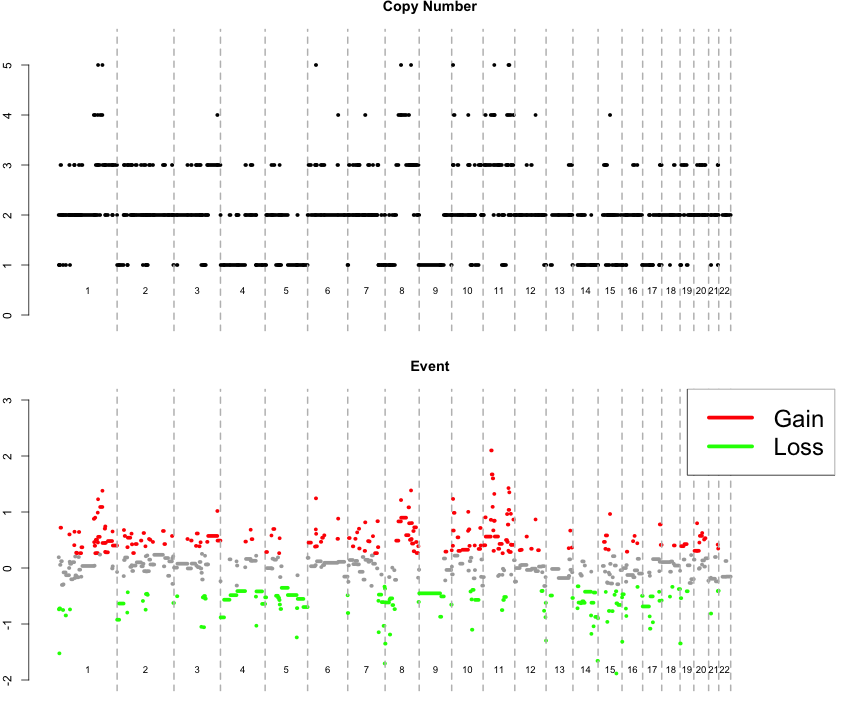
\includegraphics[width=0.75\textwidth]{figure/purity-1}
\end{center}
\caption{Correcting for sample purity and making loss/gain calls for segments.}
\label{purity}
\end{figure}

\code{SynthEx} reports copy number gain/loss event as well as integer copy number for each segment. The copy number gain/loss calls are estimated from unnormalized data, i.e., the gain/loss event is respect to the median of genome. Thus gain/loss events can be compared among different samples regardless of the ploidy of each sample. Integer copy number calls are estimated from normalized data where the baseline is diploid. For example, in a sample with whole genome doubling, a segment with copy number 2 may correspond to a copy loss event.

\subsection{Single sample analysis pipeline}
The above steps are integrated in function \code{SynthExPipeline()}. When working on multiple samples, we suggest first to run each step and choose desired model parameters and segmentation methods, and then take advantage of \code{SynthExPipeline()} to perform repetitiva analysis. The default \code{SynthExPipeline()} will report all results under \code{result.dir}.
\begin{Schunk}
\begin{Sinput}
 Segfrompipe <- SynthExPipeline(tumor, normal, bin.size = 100000,
      intersectBed.dir, genotype.file,
      result.dir, working.dir, verbose = TRUE)
\end{Sinput}
\end{Schunk}

\subsection{Without variant allele frequency}
Without variant allele frequency, \pkg{SynthEx} will only perform bias correction and segmentation.

\begin{Schunk}
\begin{Sinput}
 Segfrompipe <- SynthExPipeline(tumor, normal, bin.size = 100000,
                     intersectBed.dir, genotype.file = NULL,
                     result.dir, working.dir, verbose = TRUE)
\end{Sinput}
\end{Schunk}


\section{Multiple sample analysis}
\subsection{Batch effect and synthetic normal approach}
As shown in \pkg{SynthEx} paper, we observed strong ``batch effect" in multiple sample genomic studies. Here we demonstrate the batch effect using TCGA breast cancer dataset in \pkg{SynthEx}.
We selected top 1000 bins with largest vairance across 97 samples. Figure shows the heat map of selected bins. Each row represents a bin with mean centered at 0. Each colomn represents a sample. The corresponding dendrogram was obtained from hierarchical clustering analysis using Euclidean distance with average linkage. Several distinct patterns have been observed as if the samples are generated by different sequencing protocols. Based on our experience, such batch effect even exisits for sequencing samples from the same plate processed by the same protocols.

\begin{Schunk}
\begin{Sinput}
 normal.counts <- TCGAbreast$normal[, -c(1:3)]
 log.normal.counts <- apply(normal.counts, 2,
                            function(x){log10(x+0.01)})
 normal.var <- apply(log.normal.counts, 1, var)
 cutoff <- sort(normal.var, decreasing = TRUE)[1000]
 selected <- log.normal.counts[normal.var >= cutoff, ]
 truncated.data <- apply(selected, 1, function(x){
 	y <- x - mean(x)
 	y[y > 2] <- 2
 	y[y < -2] <- -2
 	return(y)
 })
 # each row centered at 0; data are truncated for
 # visualization purpose
 library(gplots)
 palette.gr.marray <- colorRampPalette(c("blue", "white", "red"))(56)
 heatmap.2(as.matrix(t(truncated.data)), trace = "none",
   col = palette.gr.marray, key = T, symbreaks = T, labRow = NA,
   labCol = NA, dendrogram = "column")
\end{Sinput}
\end{Schunk}

\begin{figure}
\begin{center}
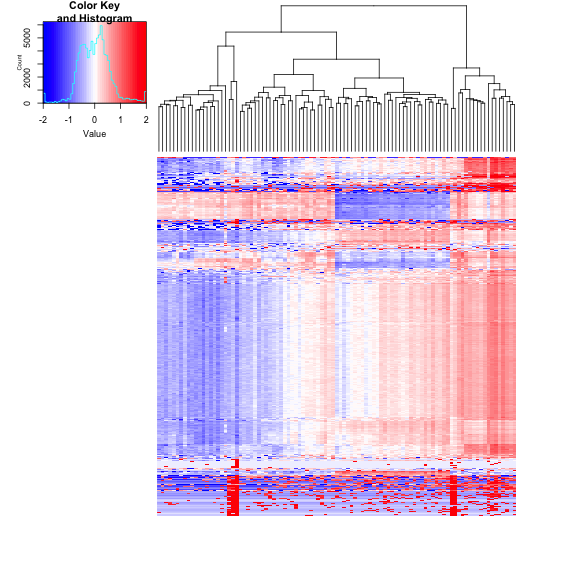
\includegraphics[width=0.8\textwidth]{figure/heatmap-1}
\end{center}
\caption{Heat map of log counts of top 1000 bins with largest vairance across 97 normal samples. Each bin is centered at 0.}
\label{heatmap1}
\end{figure}

\begin{Schunk}
\begin{Sinput}
 mm <- mean(unlist(selected))
 truncated.data2 <- apply(selected, 1, function(x){
   y <- x - mm
 	y[y > 4] <- 4
 	y[y < -4] <- -4
 	return(y)
 })
 # centered by the mean of all entries; data are truncated
 # for visualization purpose
 heatmap.2(as.matrix(t(truncated.data2)), trace = "none",
   col = palette.gr.marray, key = T, symbreaks = T, labRow = NA,
   labCol = NA, dendrogram = "column")
\end{Sinput}
\end{Schunk}

\begin{figure}
\begin{center}
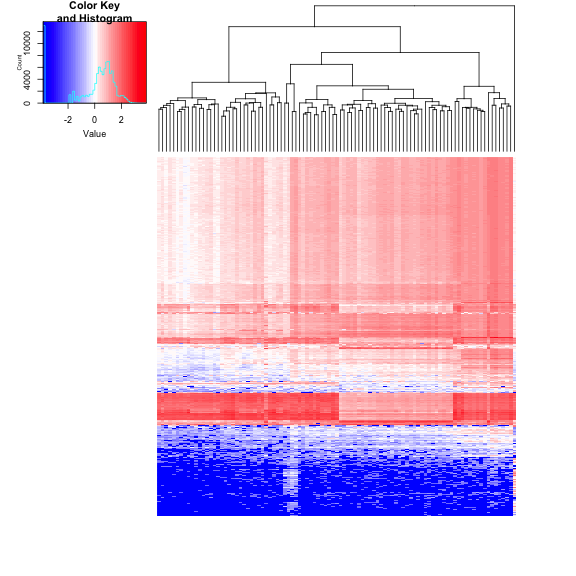
\includegraphics[width=0.8\textwidth]{figure/heatmap2-1}
\end{center}
\caption{Heat map of log counts of top 1000 bins with largest vairance across 97 normal samples. The data is centered by the mean of all elements in the log count matrix.}
\label{heatmap2}
\end{figure}

\subsection{Synthetic normal approaches}
We find using a normal smple with similar enrichment pattern (termed as synthetic normal) will lead to better result than matched normal. \pkg{SynthEx} implements different ways to generate ``synthetic normal". The most efficient way requires the input of the count of a to-be-analyzed tumor sample and a count matrix for normal samples either from the same study or from the same sequencing facility. \pkg{SynthEx} will scan through all normal samples, calcualte mean square successive variance and select $K$ normals with smallest variance. Then the synthetic normal will be generated by taking median across $K$ selected normals for each bin. The default $K$ is 1.

Here shows an example of which the segmentation gets greatly improved if using synthetic normal approach.

\begin{Schunk}
\begin{Sinput}
 tumor <- TCGAbreast$tumor[, c(1:3, 5)]
 normal <- TCGAbreast$normal[, c(1:3, 5)]
 sample.name <- colnames(TCGAbreast$tumor)[5]
 Ratio <- SynthExcorrectBias(tumor, normal, bin.size = 100000,
         rm.centromere = TRUE,
         targetAnnotateBins = NULL, saveplot = FALSE,
         centromereBins = NULL, chrX = FALSE, plot = FALSE,
         result.dir, prefix = sample.name, reads.threshold = 25)
 # Ratio <- normalization(Ratio, intersectBed.dir, genotype.file,
 # vcf = TRUE, working.dir, result.dir, cutoff = 20,
 # plot = FALSE, saveplot = FALSE, prefix = sample.name)
 # Due to the space limit, genotype file for this sample is
 # not provided.
 Seg <- createSegments(Ratio, "CBS")
 Segments <- singleCNreport(Seg, report = FALSE,
        result.dir, saveplot = TRUE,
        prefix = paste0(sample.name, "- Matched Normal"),
        plotNormalized = TRUE, WGD = 1.35,
        pos.prop.threhold = 0.6,
        pos.log2ratio.threhold = 0.75)
\end{Sinput}
\end{Schunk}

\begin{figure}
\begin{center}
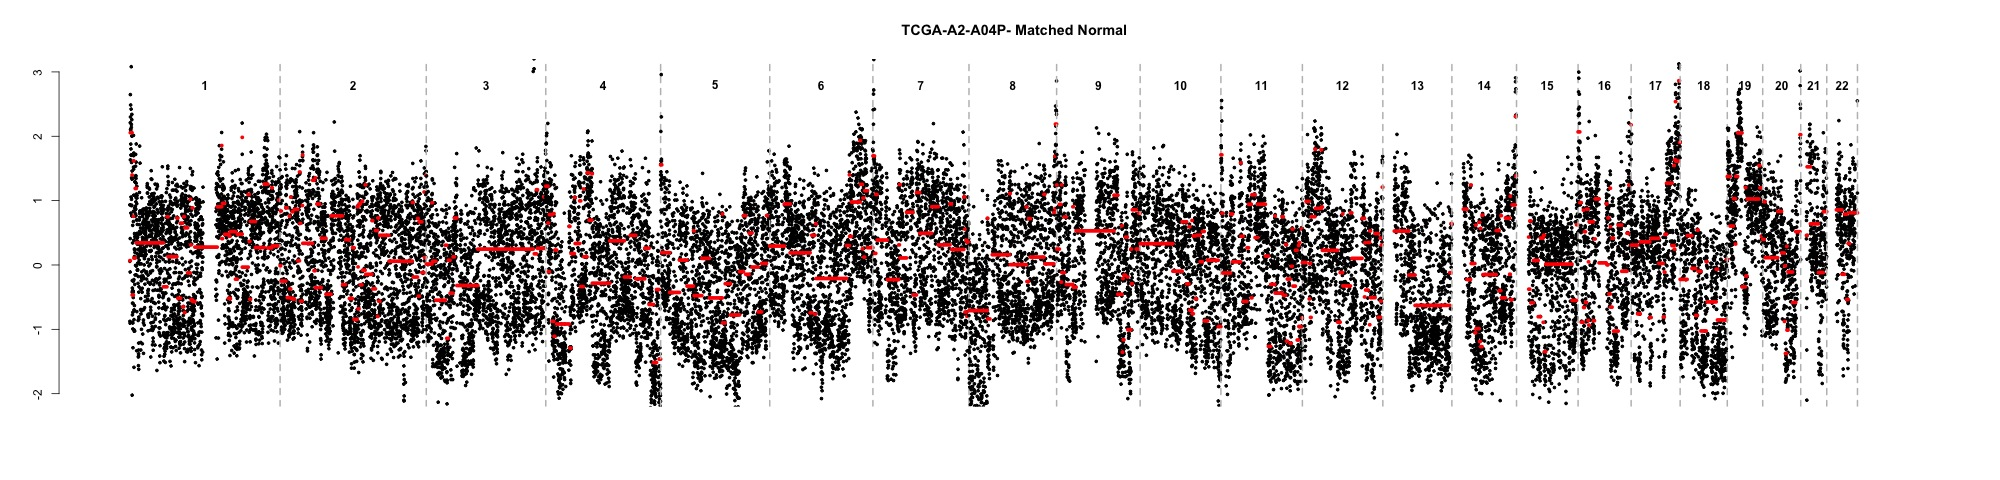
\includegraphics[width=\textwidth]{figure/multiple1-1}
\end{center}
\caption{Segmentation of TCGA-A2-A04P using matched normal.}
\label{matched}
\end{figure}

We can see the read ratio data using matched normal are very noisy. This can be fixed using the synthetic normal approach. Besides the count data of to-be-analyzed sample, \pkg{SynthEx} requires the input of the count data of a collection of normal samples (in \code{count.matrix}). These normal samples are generated using the same sequencing protocol as the to-be-analyzed tumor sample.

\begin{Schunk}
\begin{Sinput}
 tumor <- TCGAbreast$tumor[, c(1:3, 5)]
 count.matrix <- TCGAbreast$normal
 head(count.matrix[, 1:6])
\end{Sinput}
\begin{Soutput}
   chr  start    end TCGA-A1-A0SM TCGA-A2-A04P TCGA-A2-A04Q
1 chr1      0 100000          568         3135          322
2 chr1 100000 200000           22          481           40
3 chr1 200000 300000           14          224           92
4 chr1 300000 400000            0            6            6
5 chr1 400000 500000            2            0            2
6 chr1 500000 600000          101          411          152
\end{Soutput}
\end{Schunk}

\begin{Schunk}
\begin{Sinput}
 Ratio <- SynthExcorrectBias(tumor, count.matrix,
       bin.size = 100000,
       rm.centromere = TRUE,
       targetAnnotateBins = NULL, saveplot = FALSE,
       centromereBins = NULL, chrX = FALSE, plot = FALSE,
       result.dir, prefix = sample.name, reads.threshold = 25)
 #Ratio <- normalization(Ratio, intersectBed.dir,
 # genotype.file, vcf = TRUE, working.dir,
 # result.dir, cutoff = 20, plot = FALSE, saveplot = FALSE,
 # prefix = sample.name)
 # Due to the space limit, genotype file for this sample is
 # not provided.
 Seg <- createSegments(Ratio, "CBS")
 Segments <- singleCNreport(Seg, report = FALSE, result.dir,
        saveplot = TRUE,
        prefix = paste0(sample.name, "- Synthetic Normal"),
        plotNormalized = TRUE, WGD = 1.35,
        pos.prop.threhold = 0.6, pos.log2ratio.threhold = 0.75)
\end{Sinput}
\end{Schunk}

The default number of samples used to generate the synthetic normal is 1. We can change that by setting $K$. The following sample will average 10 samples with smallest variance to obtain the synthetic normal.

\begin{Schunk}
\begin{Sinput}
 sample.name <- colnames(TCGAbreast$tumor)[5]
 Ratio <- SynthExcorrectBias(tumor, count.matrix, K = 10,
         bin.size = 100000,
         rm.centromere = TRUE, targetAnnotateBins = NULL,
         saveplot = FALSE, centromereBins = NULL, chrX = FALSE,
         plot = FALSE, result.dir, prefix = sample.name,
         reads.threshold = 25)
\end{Sinput}
\end{Schunk}

\begin{figure}
\begin{center}
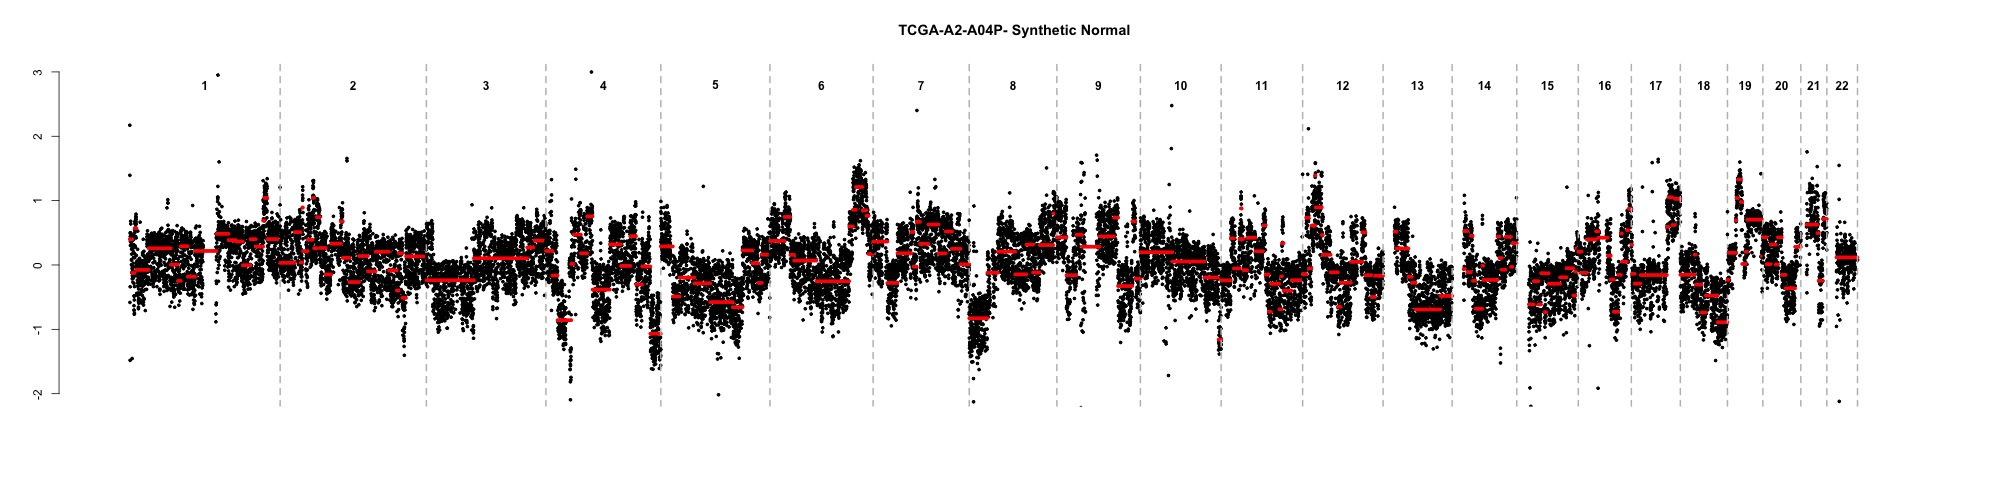
\includegraphics[width=\textwidth]{figure/multiple2-1}
\end{center}
\caption{Segmentation of TCGA-A2-A04P using synthetic normal.}
\label{synthetic}
\end{figure}

\subsubsection{Multiple sample analysis pipeline}
The above steps are integrated in function \code{SynthExPipeline()}.
\begin{Schunk}
\begin{Sinput}
 Segfrompipe <- SynthExPipeline(tumor, count.matrix,
      bin.size = 100000, intersectBed.dir, genotype.file,
      result.dir, working.dir, verbose = TRUE)
\end{Sinput}
\end{Schunk}


\subsubsection{(Optional) Creating a synthetic normal library}
The most sophisticated way to generate synthetic normal involves the assessment of quality metrics using \code{picard}. We recommend using this approach for large scale genomic studies with a sample size greater than 500 or for a sequencing facility. The construction of synthetic library requires pre-calculated fold enrichment levels of all normal samples and the groupID of each sample. Each group represents an enrichment pattern. Such grouping struture can be learned by unsupervised approach such as heatmap shown in Figure\ref{heatmap1}. Within each group, the normal samples will be stratified based on the library sizes and fold enrichment levels. The synthetic normal for a given library size and fold enrichment level is calculated as the median of all normal samples fall into that category.

\begin{Schunk}
\begin{Sinput}
 SyntheticLibrary <- create_synthetic_library(counts,
                   foldEnrichment, groupID, interval = 50000000)
 ratioCorrectedBias <- SynthExcorrectBias(tumor,
     SyntheticLibrary, bin.size = 100000, rm.centromere = TRUE,
     targetAnnotateBins = NULL, saveplot = FALSE,
     centromereBins = NULL, chrX = FALSE, plot = TRUE,
     result.dir, prefix = sample.name, reads.threshold = 25)
\end{Sinput}
\end{Schunk}

\section{Whole genome sequencing analysis}
The synthetic normal approach can be applied to whole genome sequencing(WGS) as well. Function \code{calratioWGS} can take both a matched normal sample or a count matrix of multiple normal samples. For WGS data, the step to correct for the bias in target region will be skipped. The normalization, segmentation and purity estimation step will be the same as described previously. As for segmentation, we found trend filtering outperformed others on our WGS samples. Thus we suggest to test this method on your data.
\begin{Schunk}
\begin{Sinput}
 WGSratio <- calratioWGS(tumor, normal, bin.size = 100000,
         rm.centromere = TRUE, K = 1, centromereBins = NULL,
         chrX = FALSE, reads.threshold = 25)
 Seg <- createSegments(WGSratio , "TrendFiltering")
\end{Sinput}
\end{Schunk}




\end{document}

